% ================================================================
% TEMPLATE TRABALHO - DISCIPLINA DE EQUAÇÕES DIFERENCIAIS
% ================================================================
% IMPORTANTE:
% 1. Edite este arquivo e capitulo01.bib para colocar as referências.
% - Não altere o preâmbulo deste arquivo.
% - Não coloque \documentclass, \begin{document} ou \end{document}
% - Não altere a estrutura do arquivo na parte de referencias \printbibliography 
% ================================================================

\ifdefined\LivroPrincipal
  % --------------------------------------------------------------
  \chapter{TÍTULO DO TRABALHO}
  \newcommand{\FinalizaCapitulo}{}
\else
  % --------------------------------------------------------------
  % MODO AUTÔNOMO: permite ao grupo compilar este arquivo sozinho.
  % --------------------------------------------------------------
  \documentclass[11pt,a4paper]{article}

  \usepackage[utf8]{inputenc}
  \usepackage[T1]{fontenc}
  \usepackage[brazil]{babel}
  \usepackage{lmodern}
  \usepackage{microtype}
  \usepackage{amsmath,amssymb,amsfonts,amsthm,mathtools}
  \usepackage{bm}
  \usepackage{physics}
  \usepackage{siunitx}
  \usepackage{graphicx}
  \usepackage{booktabs}
  \usepackage{array}
  \usepackage{multirow}
  \usepackage{float}
  \usepackage{caption}
  \usepackage{subcaption}
  \usepackage{enumitem}
  \usepackage{xcolor}
  \usepackage{url}
  \usepackage{hyperref}
  \usepackage{cleveref}
  \usepackage{geometry}
  \usepackage{setspace}
  \usepackage{tikz}
  \usepackage{csquotes}
  \usepackage[backend=biber,style=numeric,sorting=nyt,maxbibnames=99]{biblatex}

  \geometry{left=2.8cm,right=2.3cm,top=2.5cm,bottom=2.5cm}
  \setstretch{1.08}
  \hypersetup{colorlinks=true,linkcolor=blue,citecolor=blue,urlcolor=blue}
  \newenvironment{resumo}{\begin{center}\textbf{Resumo}\end{center}\small}{\par}\normalsize
  \addbibresource{capitulo01.bib}
  \newcommand{\FinalizaCapitulo}{\end{document}}

  \begin{document}
  \section*{TÍTULO DO TRABALHO}
  \begin{center}
  Nome Completo da Autora 1; Nome Completo da Autora 2; Nome Completo da Autora 3 (Sigam ordem de contribuição e não alfabética)
  \end{center}
\fi

\begin{resumo}
Apresente aqui, em aproximadamente 100--200 palavras, o problema estudado, o objetivo do trabalho, a metodologia utilizada, os principais resultados e a principal conclusão. Evite citações, equações longas e informações que não sejam retomadas no texto.
\end{resumo}

\noindent\textbf{Palavras-chave:} equações diferenciais; modelagem matemática; aplicações; escreva aqui mais termos relevantes.

\section{Introdução}
Apresente o problema, sua motivação e sua relevância. Explique claramente qual pergunta ou fenômeno será investigado, indique o objetivo do trabalho e contextualize a aplicação escolhida. O trabalho deve ter no \textbf{máximo 8 páginas}.

\section{Fundamentação teórica}
Apresente os conceitos matemáticos necessários para compreender o trabalho. Inclua as equações diferenciais utilizadas, hipóteses, definições, resultados teóricos, métodos analíticos e/ou numéricos e referências bibliográficas pertinentes. Toda afirmação ou resultado obtido de uma fonte externa deve ser devidamente referenciado, por exemplo~\cite{exemplo-livro}.

\subsection{Formulação matemática}
Defina as variáveis, parâmetros, condições iniciais ou de contorno e apresente o modelo matemático, como o apresentado na Equação~\eqref{eq:pvi}
\begin{equation}
\frac{dy}{dt}=f(t,y), \qquad y(t_0)=y_0.
\label{eq:pvi}
\end{equation}

As equações quando são acompanhadas de uma numeração, devem ser referenciadas em maiúsculo, isto é, deve-se utilizar Equação~\eqref{eq:pvi} ao invés de equação~\eqref{eq:pvi}. O mesmo vale para teoremas, proposições, lemas, corolários, definições, figuras e tabelas.

\subsection{Método de solução}
Descreva o método analítico ou numérico empregado. Quando pertinente, apresente algoritmo, discretização, critérios de erro e demais questões que sejam relevantes para o trabalho.

\section{Discussão dos resultados}
Apresente os resultados obtidos e discuta seu significado. Figuras e tabelas devem ser numeradas, possuir legenda e ser mencionadas no texto. Não se esqueçam que ao final da legenda sempre deve aparecer a fonte da figura, como pode ser visto na Figura~\ref{fig:exemplo}.

\begin{figure}[H]
    \centering
    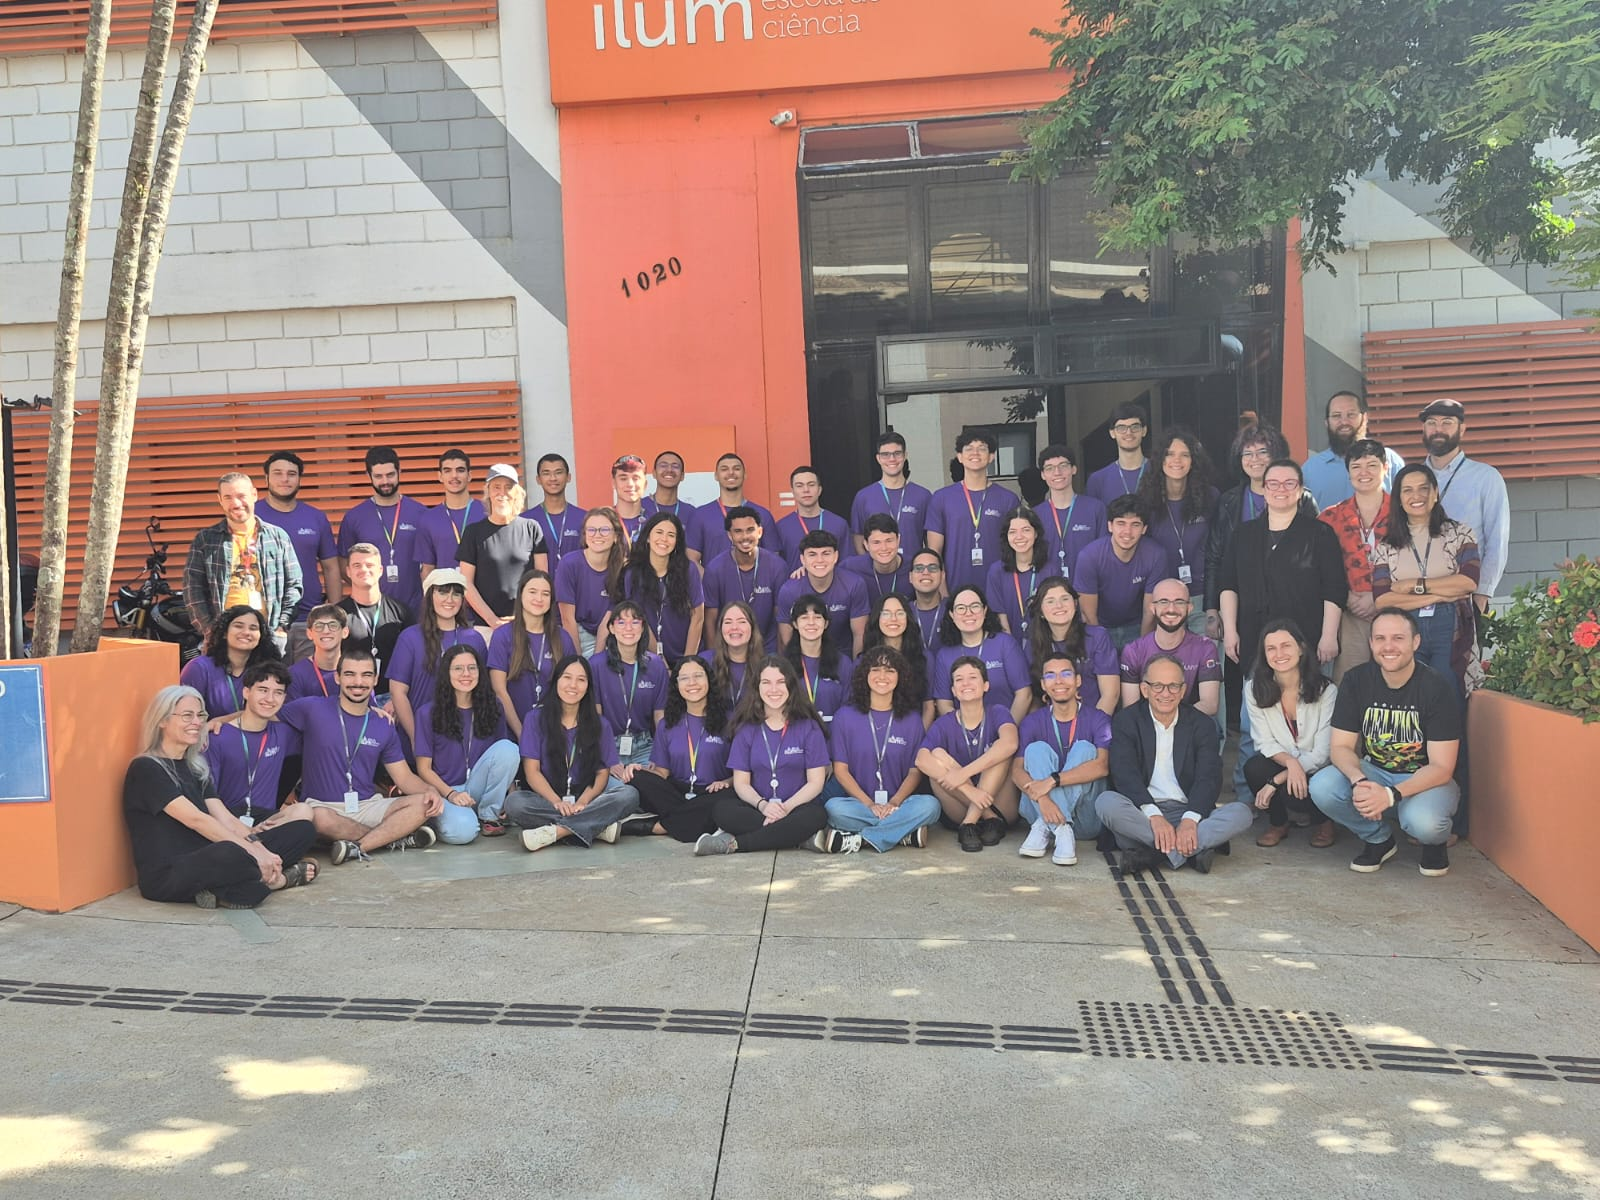
\includegraphics[width=0.9\linewidth]{Figures/t26.jpg}
    \caption{Turma 26 - Ilum Escola de Ciência. Fonte: Documentos oficiais da Ilum \url{https://ilum.cnpem.br/noticias_e_eventos/}}
    \label{fig:exemplo}
\end{figure}



Compare os resultados com a teoria, discuta limitações, comportamento do modelo, interpretações, erros de aproximação e demais informações relevantes para o trabalhos. Se for o caso, utilizem tabelas para auxiliar na organização da informação, como o modelo apresentado na Tabela~\ref{tab:exemplo}.

\begin{table}[H]
\centering
\caption{Exemplo de tabela.}
\label{tab:exemplo}
\begin{tabular}{lcc}
\toprule
Método & Erro & Tempo \\
\midrule
Método A & 0,00 & 0,00 \\
Método B & 0,00 & 0,00 \\
\bottomrule
\end{tabular}
\end{table}

\section{Considerações finais}
Retome o objetivo do trabalho e apresente as principais conclusões. Destaque o que foi aprendido sobre o problema e sobre o uso de equações diferenciais na aplicação estudada. Não introduza resultados novos nesta seção. Perspectivas futuras são bem vindas, mas não obrigatórias.

\section{Contribuição de cada autor}
Descreva objetivamente a participação de cada integrante. A descrição deve permitir identificar a contribuição individual de cada autor, incluindo, conforme o caso, revisão bibliográfica, formulação matemática, implementação computacional, análise dos resultados, produção de figuras e tabelas, redação e revisão do texto. \textbf{Utilizem essas informações para definir a ordem de autoria do trabalho}, isto é, a ordem deve ser da pessoa que mais contribuiu para aquela que menos contribuiu.

\begin{itemize}[leftmargin=*]
    \item Nome do Autor 1: descreva a contribuição.
    \item Nome do Autor 2: descreva a contribuição.
    \item Nome do Autor 3: descreva a contribuição, se houver.
\end{itemize}

% ================================================================
% Não altere esta parte.
% ================================================================
\ifdefined\LivroPrincipal
\else
  \printbibliography[heading=bibintoc,title={Referências}]
\fi
\FinalizaCapitulo

\end{document}